\newcommand{\chapter}[2][]{
	\newcommand{\chapname}{#2}
	\begin{flushleft}
		\begin{minipage}[t]{\linewidth}
			
\includegraphics[height=1cm]{hdht-logo.png}
			\hspace{0pt}	
			\sffamily\bfseries\large Bài  15.
			\begin{flushleft}
				\huge\bfseries #1
			\end{flushleft}
		\end{minipage}
	\end{flushleft}
	\vspace{1cm}
	\normalfont\normalsize
}
\chapter[Ba định luật Newton về chuyển động]{Ba định luật Newton về chuyển động}
\section{Lý thuyết}

\subsection{Định luật I Newton về chuyển động}
\subsubsection{Nội dung định luật}
Nếu một vật không chịu tác dụng của lực nào hoặc chịu tác dụng tác dụng của các lực có hợp lực bằng không, thì vật đang đứng yên sẽ tiếp tục đứng yên, đang chuyển động sẽ tiếp tục chuyển động thẳng đều.
\subsubsection{Quán tính}
Quán tính là tính chất của mọi vật có xu hướng bảo toàn vận tốc cả về hướng và độ lớn.
Định luật I được gọi là định luật quán tính và chuyển động thẳng đều được gọi là chuyển động theo quán tính.
\subsection{Định luật II Newton về chuyển động}
\subsubsection{Nội dung định luật}
Gia tốc của một vật cùng hướng với lực tác dụng lên vật. Độ lớn của gia tốc tỉ lệ thuận với độ lớn của lực và tỉ lệ nghịch với khối lượng của vật.
\begin{equation*}
	\vec{a}=\dfrac{\vec F}{m},
\end{equation*}
trong đó:
\begin{itemize}
	\item $\vec F$ là lực tác dụng lên vật (N);
	\item m là khối lượng của vật (kg);
	\item $\vec a$ là gia tốc của vật ($\text{m/s}^2$).
\end{itemize}

\subsubsection{Khối lượng và quán tính}
Khối lượng là đại lượng đặc trưng cho mức quán tính của vật. Vật có mức quán tính lớn hơn thì khối lượng lớn hơn và ngược lại. 

\subsubsection{Trọng lực - Trọng lượng}

Trọng lực là lực của Trái Đất tác dụng vào vật gây ra cho chúng gia tốc rơi tự do. Trọng lực kí hiệu là $\vec P.$

Ở gần Trái Đất, trọng lực có phương thẳng đứng, có chiều từ trên xuống và đặt vào một điểm đặc biệt của mỗi vật, gọi là trọng tâm của vật.

Độ lớn của trọng lực tác dụng lên một vật gọi là trọng lượng của vật, kí hiệu là $P$. 

Công thức tính trọng lực: 
\begin{equation*}
	\vec P=m\vec g.
\end{equation*}
\subsection{Định luật III Newton về chuyển động}
\subsubsection{Nội dung định luật}
Trong mọi trường hợp, khi vật A tác dụng lên vật B một lực, thì vật B cũng tác dụng lại vật A một lực. Hai lực này có cùng giá, cùng độ lớn, nhưng ngược chiều.
\begin{equation*}
	{\vec F}_{\text{AB}}=-{\vec F}_{\text{BA}}.
\end{equation*}
\subsubsection{Lực và phản lực}
Một trong hai lực tương tác giữa hai vật gọi là lực tác dụng còn lực kia gọi là phản lực.

Lực và phản lực có những đặc điểm: 
\begin{itemize}
	\item Lực và phản lực luôn luôn xuất hiện (hoặc mất đi) đồng thời.
	\item Lực và phản lực có cùng giá, cùng độ lớn nhưng ngược chiều. Hai lực có đặc điểm như vậy gọi là hai lực trực đốkhông cân bằng nhau vì chúng đặt vào hai vật khác nhau.
\end{itemize}
\subsection{Chuyển động của vật và hệ vật}
Nếu các vật trong hệ liên kết với nhau bằng dây nối, dây không giãn, nhẹ thì các vật trong hệ chuyển động với cùng một gia tốc

\begin{equation*}
	\vec a = \dfrac{\vec F_1 + \vec F_2 + ...}{m_1 + m_2+...}
\end{equation*}

Nếu các vật liên kết với nhau bằng ròng rọc cần chú ý:
\begin{itemize}
\item Đầu dây luồn qua ròng rọc động đi được quãng đường $s$ thì vật treo vào trục ròng rọc đi được quãng đường là $\dfrac{s}{2}$, vận tốc và gia tốc cũng theo tỉ lệ đó.

\item Nếu hệ gồm hai vật chồng lên nhau thì khi có chuyển động tương đối ta cần khảo sát từng vật riêng lẻ, khi không có chuyển động tương đối ta coi hai vật là một vật có khối lượng bằng tổng khối lượng của hai vật khi khảo sát.
\end{itemize}
\section{Mục tiêu bài học - Ví dụ minh họa}
\begin{dang}{Ghi nhớ định luật I Niu-tơn. \\ Nhận biết quán tính}
	\viduii{1}{Một chiếc xe buýt đang chạy trên đường thì tài xế phanh xe gấp. Một hành khách ngồi ở cuối xe phàn nàn rằng, do bác tài xế phanh xe gấp mà chiếc túi xách ở phía trước bay về phía anh ta làm anh ta bị đau. Người hành khách nói đúng hay sai? Em hãy giải thích?
	}
	{	\begin{center}
			\textbf{Hướng dẫn giải}
		\end{center}
		
		Người hành khách đã nói sai. Khi xe dừng lại đột ngột, túi xách theo quán tính phải bay về phía trước, không phải bay về phía sau.
		
	}
	\viduii{1}{\begin{enumerate}[label=\alph*.]
			\item Em hãy giải thích tại sao khi ta nhảy từ bậc cao xuống chân ta bị gập lại.  	
			\item Khi cán búa lỏng, tại sao ta có thể làm chặt lại bằng cách gõ mạnh đuôi cán xuống đất.
		\end{enumerate}
	}
	{	\begin{center}
			\textbf{Hướng dẫn giải}
		\end{center}
		
		\begin{enumerate}[label=\alph*.]
			\item Nhảy từ bậc cao xuống, chân chạm đất bị dừng lại ngay, nhưng người còn tiếp tục chuyển động theo quán tính nên làm chân gập lại.  	
			\item Khi gõ mạnh đuôi cán búa xuống đất, cán búa đột ngột dừng lại. Do quán tính đầu búa tiếp tục chuyển động gắn chặt vào cán búa. 
		\end{enumerate}
	}
\end{dang}	
\begin{dang}{Ghi nhớ định luật II Niu-tơn}
	\viduii{1}{Trong các cách viết công thức của định luật II Niu - tơn sau đây, cách viết nào đúng?
		\begin{mcq}(2)
			\item $- \vec{F} = m\vec{a}$.
			\item $\vec{F} = m\vec{a}$. 
			\item $\vec{F} = - m\vec{a}$.
			\item $\vec{F} = ma.$
		\end{mcq}
	}
	{	\begin{center}
			\textbf{Hướng dẫn giải}
		\end{center}
		
		Gia tốc của một vật cùng hướng với lực tác dụng lên vật. Độ lớn của gia tốc tỉ lệ thuận với độ lớn của lực và tỉ lệ nghịch với khối lượng của vật.
		\begin{equation*}
			\vec{a}=\dfrac{\vec F}{m},
		\end{equation*}
		
		\textbf{Đáp án: B}
	}
	\viduii{1}{Chọn câu phát biểu đúng?
		\begin{mcq}
			\item Nếu không có lực tác dụng vào vật thì vật không chuyển động được. 
			\item Lực tác dụng luôn cùng hướng với hướng biến dạng. 
			\item Vật luôn chuyển động theo hướng của lực tác dụng. 
			\item Nếu có lực tác dụng lên vật thì vận tốc của vật bị thay đổi.
		\end{mcq}	
	}
	{	\begin{center}
			\textbf{Hướng dẫn giải}
		\end{center}
		
		Lực gây ra gia tốc làm thay đổi vận tốc của vật.
		
		
		\textbf{Đáp án: D}
	}
\end{dang}
\begin{dang}{Ghi nhớ định luật III Niu-tơn, đặc điểm của cặp lực - phản lực}
	\viduii{1}{Trong một vụ tai nạn, một ô tô tải đâm vào một ô tô con đang chạy ngược chiều. Ô tô nào chịu lực lớn hơn? Hãy giải thích.
	}
	{	\begin{center}
			\textbf{Hướng dẫn giải}
		\end{center}
		
		Theo định luật III Niu-tơn , ô tô tải tác dụng vào ô tô con một lực thì ô tô con cũng tác dụng ngược lại ô tô tải một lực.Hai ô tô chịu lực bằng nhau về độ lớn,cùng phương nhưng ngược chiều nhau. Vì vậy, hai ô tô đều chịu một lực có độ lớn bằng nhau.
		
	}
	\viduii{1}{Khi đi bộ xa hoặc leo núi, ta chống gậy thì đỡ mỏi  chân. Tại sao?
		
	}
	{	\begin{center}
			\textbf{Hướng dẫn giải}
		\end{center}
		
		Khi đi bộ hoặc leo núi, chân ta phải đạp vào mặt đất, đất sẽ tác dụng một phản lực làm cho ta đi được. Động tác đó lặp đi lặp lại nhiều lần khiến cho cơ chân bị mỏi. Khi chống gậy, ta dùng tay ấn mạnh gậy về phía sau, mặt đất sẽ tác dụng vào đầu gậy một phản lực hướng về phía trước. Phản lực này sẽ truyền qua gậy đến cơ thể làm cho ta dịch chuyển về phía trước. Như vậy đã thay bớt hoạt động của chân bằng hoạt động của tay nên chân đỡ mỏi hơn.
	}
\end{dang}

\begin{dang}{Thực hiện áp dụng định luật III Niu-tơn}
	\viduii{3}{Một A vật có khối lượng $\SI{1}{kg}$ chuyển động với tốc độ $\SI{5}{m/s}$ va chạm vào một vật B đứng yên. Sau va chạm vật A chuyển động ngược trở lại với tốc độ $\SI{1}{m/s}$, còn vật B chuyển động với tốc độ $\SI{2}{m/s}$. Hỏi khối lượng của vật B bằng bao nhiêu?
	}
	{	\begin{center}
			\textbf{Hướng dẫn giải}
		\end{center}
		
		Chọn chiều dương là chiều chuyển động của vật A
		
		$$ F_{21} = -F_{12} \Leftrightarrow m_1 a_1 = - m_2a_2.$$
		
		$$ \Rightarrow m_1 \dfrac{\Delta v_1}{\Delta t} = m_2 \dfrac{\Delta v_2}{\Delta t}.$$
		
		Suy ra $m_2 = \SI{3}{kg}.$
		
	}
	\viduii{3}{Một quả bóng, khối lượng $\SI{500}{g}$ bay với tốc độ $\SI{20}{m/s}$ đập vuông góc vào bức tường và bay ngược lại với tốc độ $\SI{20}{m/s}$. Thời gian va đập  là $\SI{0,02}{s}$. Lực do bóng tác dụng vào tường có độ lớn và hướng như thế nào?		
	}
	{	\begin{center}
			\textbf{Hướng dẫn giải}
		\end{center}
		
		Chọn chiều dương chuyển động là chiều bóng bay đập vào tường.
		
		Gia tốc mà quả bóng đạt được là
		
		$$a = \dfrac{v-v_0}{t} = \SI{2000}{m/s^2}.$$
		
		Lực do quả bóng tác dụng vào tường là
		
		$$F =ma = \SI{1000}{N}.$$
		
		Có cùng hướng chuyển động ban đầu của bóng.	
	}
	
\end{dang}
\begin{dang}{Thực hiện biểu diễn tất cả các lực tác dụng lên vật hoặc hệ hai vật chuyển động, tính gia tốc và các đại lượng trong công thức của các định luật Niu-tơn để viết phương trình chuyển động cho vật hoặc \\hệ vật}
	\viduii{3}{Hai vật $m_1 = \SI{1}{kg}$, $m_2 = \SI{0,5}{kg}$ nối với nhau bằng sợi dây và được kéo lên thẳng đứng nhờ lực $F = \SI{18}{N}$ đặt lên vật I. Tìm gia tốc chuyển động và lực căng của dây. Coi dây là không giãn và có khối lượng không đáng kể.
		\begin{center}
			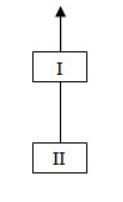
\includegraphics[scale=0.8]{../figs/VN10-PH-12-A-003-1-V2-01.jpg}
		\end{center}
	}
	{	\begin{center}
			\textbf{Hướng dẫn giải}
		\end{center}
		\begin{center}
			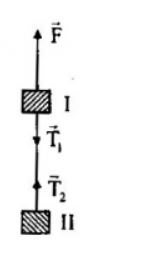
\includegraphics[scale=0.8]{../figs/VN10-PH-12-A-003-1-V2-02.jpg}
		\end{center}
		Các ngoại lực tác dụng lên hệ: $\vec P_1; \vec P_2; \vec F$.
		
		Chọn chiều dương hướng lên. Gia tốc của hệ
		
		$$a = \dfrac{F - \vec P_1 - vec P_2}{m_1+m_2} = \dfrac{F - m_1g -m_2g}{m_1 + m_2} = \SI{2}{m/s^2}.$$
		
		Xét riêng vật $m_2$, ta có: 
		
		$$T - P_2 = m_2a \Rightarrow T =m_2a + P_2 = m_2 (a+g) \Rightarrow T = \SI{6}{N}.$$
		
		
		
		
	}
	\viduii{3}{Một vật khối lượng $m$ treo vào trần một thang máy khối lượng $M$, $m$ cách sàn thang máy một khoảng $s$. Tác dụng lên buồng thang máy lực $F$ hướng lên.
		\begin{enumerate}[label=\alph*]
			\item Tính gia tốc của $m$ và lực căng dây treo.
			\item Dây đứt đột ngột. Tính gia tốc của vật và buồng thang máy sau khi dây đứt và thời gian từ lúc đứt dây đến lúc vật $m$ chạm sàn.
		\end{enumerate}
		
	}
	{	\begin{center}
			\textbf{Hướng dẫn giải}
		\end{center}
		
		\begin{center}
			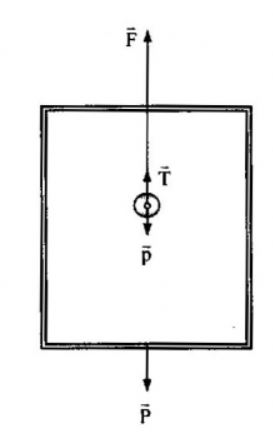
\includegraphics[scale=0.5]{../figs/VN10-PH-12-A-003-1-V2-03.jpg}
		\end{center}
		
		\begin{enumerate}[label=\alph*]
			\item Gia tốc của $m$ và lực căng của dây treo
			
			- Chọn chiều dương hướng lên.
			
			- Các ngoại lực tác dụng lên hệ "thang máy và người" là: lực $\vec F$, các trọng lực $\vec P$, $\vec p$. Theo định luật II Niu - tơn:
			
			$$\vec F + \vec P + \vec  p = (M+m)\vec a.$$
			
			$$ a =\dfrac{F - (M+m)g}{M+m}.$$
			
			- Xét riêng vật $m$
			
			$$T - p =ma \Rightarrow T = m(g+a) \Rightarrow T = \dfrac{mF}{M+m}.$$
			
			\item Gia tốc của vật và buồng thang máy sau khi đứt dây và thời gian từ lúc dây đứt đến lúc $m$ chạm sàn.
			
			- Khi đứt dây: $F =0 \Rightarrow a_2 =-g$: vật $m$ không gắn với thang máy nữa nên $a_1 = \dfrac{F}{M} - g.$
			
			- Thời gian từ lúc dây đứt đến lúc chạm sàn:
			
			+ Chọn hệ quy chiếu gắn với thang máy. 
			
			$$a' =a_1 +g = \dfrac{F}{M}$$.
			
			+ Thời gian rơi của $m$ khi dây đứt là:
			
			$$ t=\sqrt {\dfrac{2s}{a'}} = \sqrt{\dfrac{2sM}{F}}.$$
			
			
		\end{enumerate}	
	}
	
	\viduii{3}{Cho hệ vật như hình vẽ có $m_1 = 2m_2$. Lực căng của dây treo ròng rọc là $\SI{52,3}{N}$. Tìm gia tốc chuyển động của mỗi vật, lực căng của dây treo vật. Lấy $g = \SI{9,8}{m/s^2}$.
		
		\begin{center}
			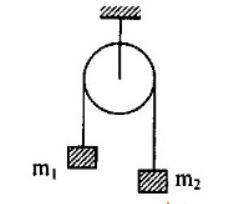
\includegraphics[scale=0.5]{../figs/VN10-PH-12-A-003-1-V2-04.jpg}
		\end{center}
	}
	{	\begin{center}
			\textbf{Hướng dẫn giải}
		\end{center}
		\begin{center}
			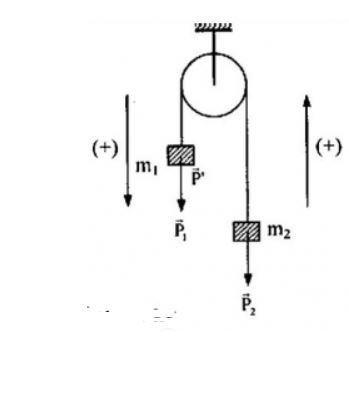
\includegraphics[scale=0.6]{../figs/VN10-PH-12-A-003-1-V2-05.jpg}
		\end{center}
		- Vì bỏ qua khối lượng ròng rọc nên: 
		
		$$ T' = 2T \Rightarrow T = \dfrac{T'}{2} = \SI{26,15}{N}.$$
		
		- Do $m_1 > m_2$ nên $m_1$ đi xuống, $m_2$ đi lên. Chọn chiều dương là chiều chuyển động của hệ.
		
		
		Áp dụng định luật II Niu - tơn:
		
		$$\vec P_1 + \vec P_2 =(m_1 + m_2) \vec a.$$
		
		Chiếu biểu thức trên lên chiều dương đã chọn:
		
		$$P_1 - P_2 =(m_1+m_2)a \Rightarrow a = \dfrac{m_1 - m_2}{m_1 +m_2} g= \dfrac{2m_2 -m_2}{2m_2 + m_2}g	= \SI{3,27}{m/s^2}.$$	
		
		- Xét riêng vật $m_2$ 
		
		$$T - P_2 =m_2a \Rightarrow T -m_2g = m_2a \Rightarrow m_2 = \dfrac{T}{g+a} = \SI{2}{kg}.$$
		
		Suy ra $m_1 =2m_2 = \SI{4}{kg}.$
	}
	
\end{dang}